\documentclass[a4paper, 11pt]{article}
\usepackage{comment}
\usepackage{fullpage}
\usepackage{amsmath}
\usepackage{amssymb}
\usepackage{mathtools}
\usepackage{fontspec}
\usepackage{siunitx}
\defaultfontfeatures{Ligatures=TeX}
\usepackage{xfrac}
\usepackage{icomma}
\usepackage[section,below]{placeins}
\usepackage[labelfont=bf,font=small,width=0.9\textwidth]{caption}
\usepackage{subcaption}
\usepackage{graphicx}
\usepackage{grffile}
\usepackage{float}
\floatplacement{figure}{htbp}
\floatplacement{table}{htbp}
\usepackage{booktabs}
\usepackage{hyperref}
\begin{document}
\noindent
\centerline{\small{\textsc{Michigan State University}}} \\
\large{\textbf{CMSE/CSE 822 – Parallel Computing \hfill Fall 2019 \\
Homework 2}} \\
Alexander Harnisch \\
\noindent\makebox[\linewidth]{\rule{\textwidth}{0.4pt}}

\section*{1) Performance Modeling}
\subsection*{a)}
\label{sec:1a}
There is some missing information here and assumptions have to be made.
However, it's not important since it only effects the numbers to plug in and
get out, not the logic behind it.

The kernel performs 6 floating point operations (FLOP) in each iteration.
Assuming no caching we have seven floating point number reading and one writing
operation for each loop iterations. However, we can assume that the same
variables are kept in the registers in each loop iterations, or at least in
fast memory. Which means the entire $y$ and $z$ arrays both only have to be
loaded once. Assuming single precision with $\SI{4}{byte}$ per float that
translates to $\SI{12}{byte}$ of memory access and an arithmetic intensity $I$
of
\begin{equation}
  I = \frac{\SI{6}{FLOP}}{\SI{12}{byte}} = \frac{1}{2}\,\frac{\textup{FLOP}}{\textup{byte}}\,.
\end{equation}

\subsection*{b)}
In a simple roofline model for some $I$ the critical peak performance
$\pi_\textup{crit}$ is given by $\beta I$, where $\beta$ is the peak memory
bandwidth. So for $I = 0.5\,\frac{\textup{FLOP}}{\textup{byte}}$ from
\hyperref[sec:1a]{a)} we get:
\begin{equation}
  \pi_\textup{crit} = 30\,\frac{\textup{GB}}{\textup{s}}\cdot \frac{1}{2}\,\frac{\textup{FLOP}}{\textup{byte}} = 15\,\frac{\textup{GFLOP}}{\textup{s}}\,.
\end{equation}
So in case the processor's peak performance is greater than
$\SI{15}{GFLOP\per\second}$ the kernel is compute bound, otherwise
memory bound.

\newpage
\subsection*{c)}
A simple roofline model plot is given by Figure~\ref{fig:roofline}. The
performance for an arithmetic intensity of $I = \SI{0.5}{FLOP\per byte}$ is
$\SI{15}{GFLOP\per\second}$.
\begin{figure}
  \centering
  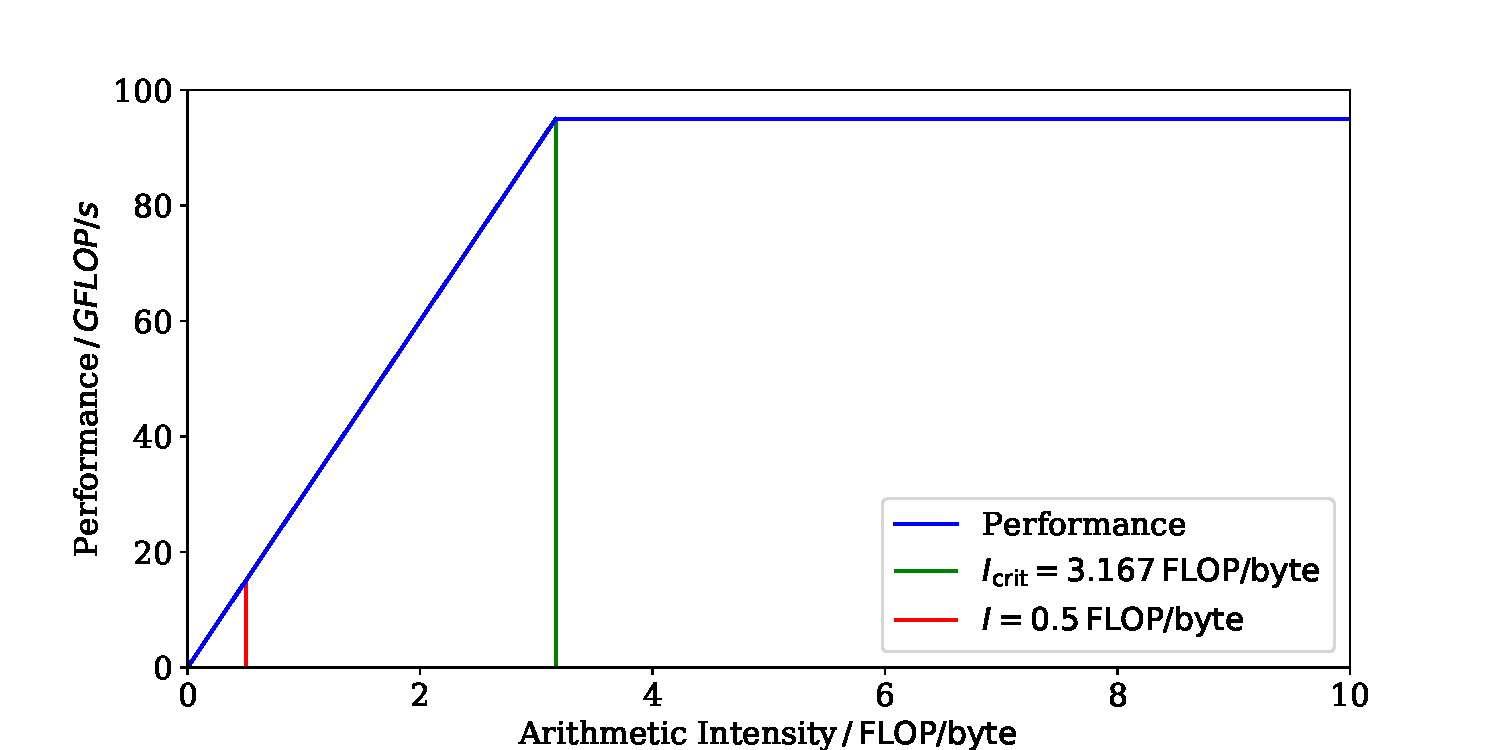
\includegraphics[width=\textwidth]{../plot/roofline.pdf}
  \caption{Simple roofline model.}
  \label{fig:roofline}
\end{figure}

\section*{2) Cache optimization: Matrix Vector Multiplication}

\textbf{General Comment:} I am very interested in fully understanding what is
going on here. However, I simply don't have the time to properly think about
all the plots I've generated. I keep exact track of how I spend my productive
time, partly to point out to professors when their homework takes up more time
than it is supposed to. I spent \SI{28}{hours} in total on this homework (and
almost all of it on the second part). This is simply too much. Yes I did a few
things that are definitely beyond of what was asked for, but without it it
seemed very hard to get any reliable data. This was also partly due to the
first published version of the homework being very confusing and it being
updated after I already waisted 10 hours of my time on it. The available time
for the homework for this class in a graduate student's weekly schedule
(assuming a 40 hour work week) is 3 hours and 40 minutes on average over the
entire duration of the class. In other words: This week's assignment was about
a factor of 7.7 longer than what it is supposed to. MSU claims to care about
student's mental health, so please act like it and keep that in mind for future
assignments.

\subsection*{a) Implementation}
See code in repository.

\subsection*{b) and c) Performance Analysis and Cache Performance Measurement}
For all of the testing in this subsection, I wrote scripts for fully automated
job submission and data collection  in \textsc{Bash} and \textsc{Python}. Using
this system, I tested $4432$ different sets of parameters ($N$, $M$ and $B$).
For each run the relative speedup as well as cache misses for L1, L2 and L3
were collected. All of the results are summarized in the following plots. The
raw data can be found in the file \textit{data.txt} in my repository, outside
of the submission directory.

Figure~\ref{fig:all_runs} shows the speedup for all tested matrices in
dependence of the blocking factor $B$. Each data point is the average speedup
for all matrices with the corresponding $B$ value. This was the first data I
looked at, also splitting it down by matrix sizes, to get a general feel for
the data and choose a reasonable blocking factor for tests with fixed blocking
factors and varied matrix shape. $B = 200$ was chosen for that, also because it
lays within the window of highest speedup in Figure~\ref{fig:square_against_B}.
\begin{figure}
  \centering
  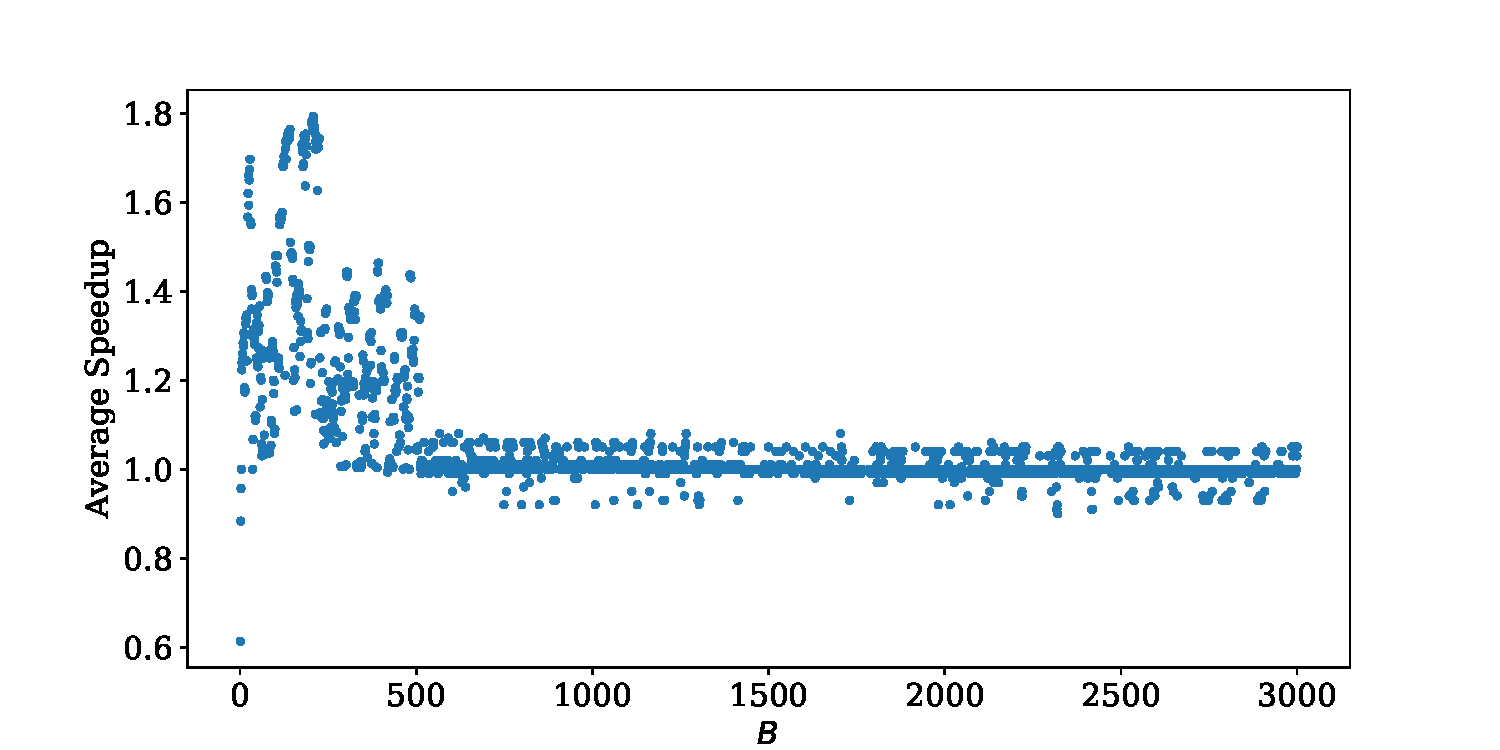
\includegraphics[width=\textwidth]{../plot/speedup_for_all_bs.pdf}
  \caption{Average speedup for all tested matrices in dependence of the blocking factor $B$.}
  \label{fig:all_runs}
\end{figure}
\FloatBarrier

Figure~\ref{fig:square_against_B} is probably the most insightful one. It shows
the achieved speedup and ratio of cache misses for all blocking factors between
0 and 512 for a constant matrix shape of $N = M = 10000$. This plot has many
interesting features, many of which I do not understand (for example: there is
a periodicity in L1 misses for $B>285$ that also periodically effects L3 misses
and speedup).
\begin{figure}
  \centering
  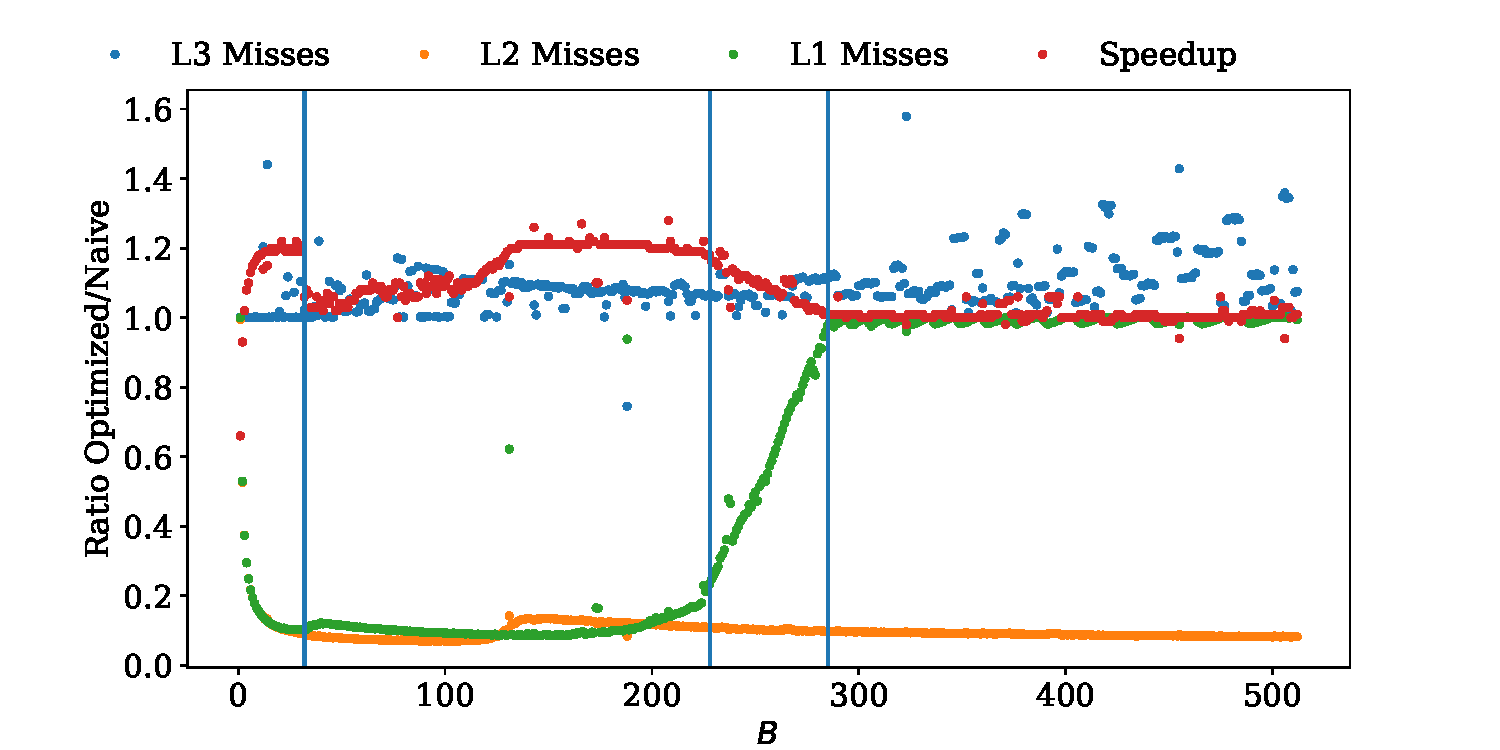
\includegraphics[width=\textwidth]{../plot/square_against_B.pdf}
  \caption{Results for a fixed matrix size of $N = M = 10000$ for different
  blocking factors $B$. For reference, the plot includes blue vertical lines
  at $B=32$, $B=228$ and $B=285$.}
  \label{fig:square_against_B}
\end{figure}

We can clearly see a correlation between L1 cache miss rate and speedup. For $B
> 228$ the L1 cache seems to be too small for the blocking and it starts to
become less and less effective for larger blocking factors. We can see how the
speedup slowly declines back to one as the L1 cache miss rate increases and the
ratio approaches one, in which case there is practically no difference between
the naive and optimized implementation any more as all of the cached values
have been overwritten once they are needed again.

However, for some reason the L2 miss rate still seems to be significantly lower
for the optimized method without any significant speedup, which I do not fully
understand. My best guess is that the L2 latency is just too high for the
achieved changes in L2 miss rate to have any significant effect on speedup in
this scenario. We can find more evidence for this hypothesis in my other plots,
which also do not show a significant correlation between L2 miss rate and
speedup (see Figure~\ref{fig:fixed_B_different_squares} and
Figure~\ref{fig:fixed_B_N_different_M}).

It is also unclear why there is no observable speedup for $32 < B < 125$
despite the L1 and L2 miss rate being consistently low. Maybe it has to do with
cache latency and overhead due to the added loops. The initial rise in speedup
is cut off by a drop at exactly $B = 32$, which is probably related to a lower
cache latency with a cache block size of 32. But then there should be a similar
effect for $B = 64$, which there is not.

\FloatBarrier
\begin{figure}
  \centering
  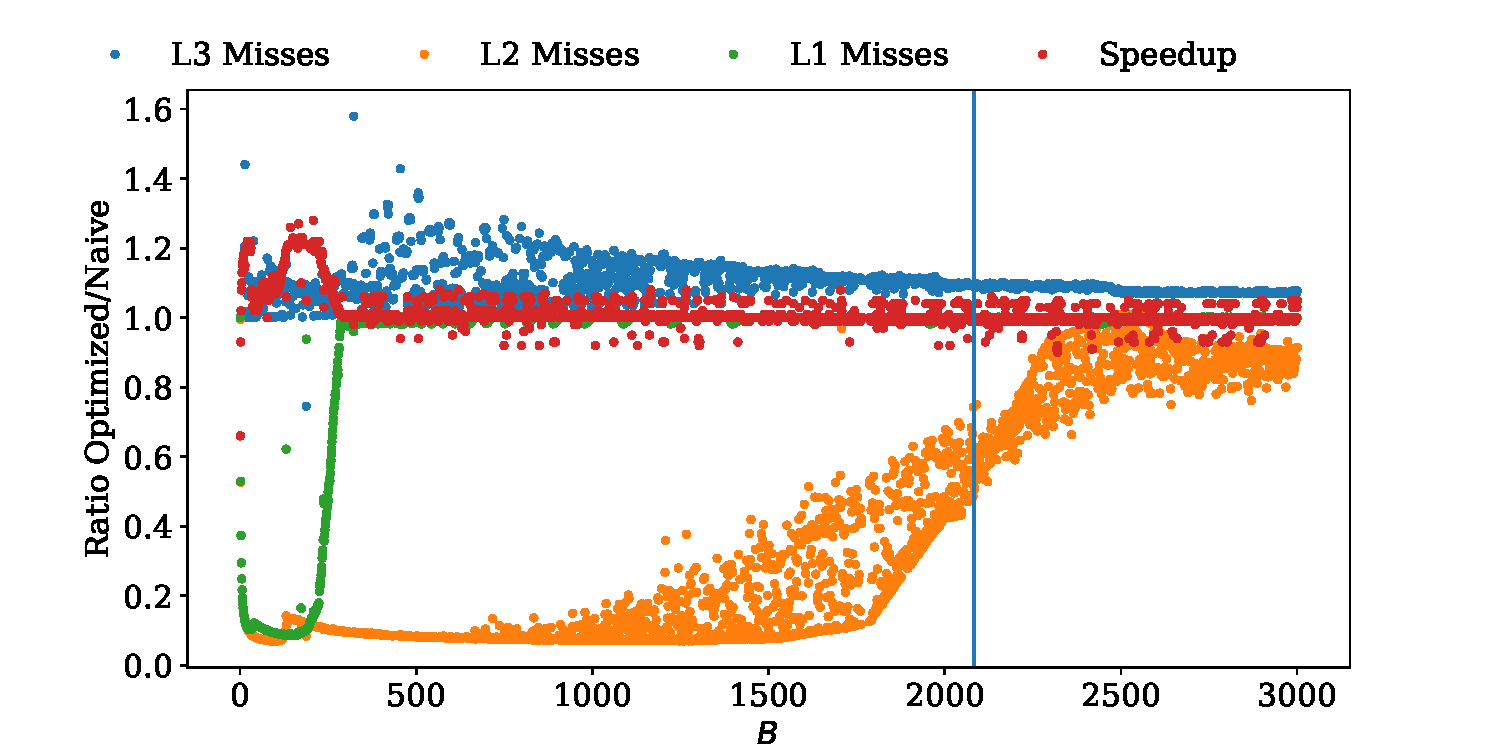
\includegraphics[width=\textwidth]{../plot/square_against_B_L2.pdf}
  \caption{Results for a fixed matrix size of $N = M = 10000$ for different
  blocking factors $B$. For reference, the plot includes a blue vertical line
  at $B=2083$.}
  \label{fig:square_against_B_L2}
\end{figure}
To start seeing L2 cache misses we have to test larger blocking factors. For
that purpose, Figure~\ref{fig:square_against_B_L2} is an extension of
Figure~\ref{fig:square_against_B} with blocking factors up to $B=3000$. We can
clearly make out the rising edge of L2 cache misses. However, as mentioned
before L2 cache misses have no effect on performance in this setting. The
middle of the rising edge can be found at $B=2083$.

\FloatBarrier
\begin{figure}
  \centering
  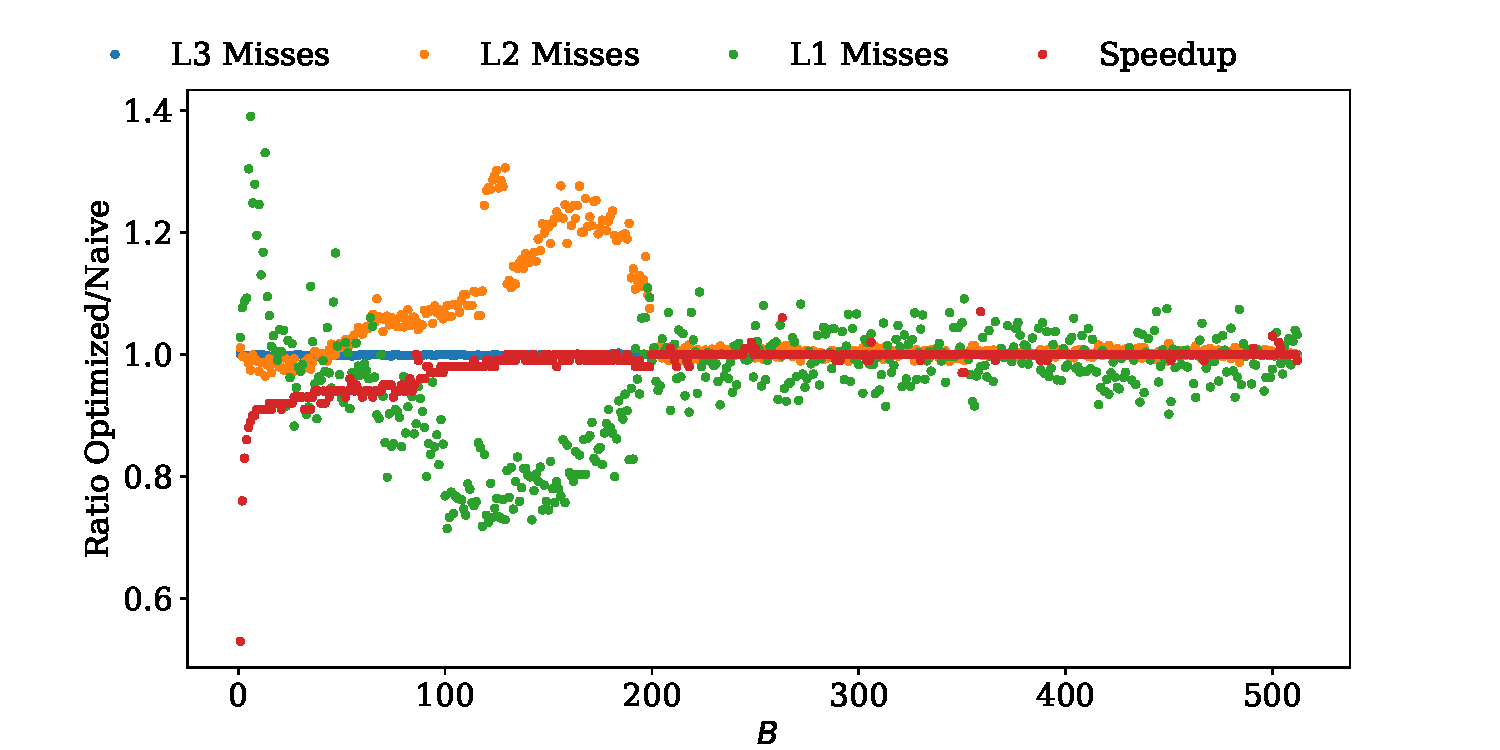
\includegraphics[width=\textwidth]{../plot/narrow_against_B.pdf}
  \caption{Results for a narrow matrix with $N=100000$ and $M=200$ for different blocking factors $B$.}
  \label{fig:narrow_against_B}
\end{figure}

\begin{figure}
  \centering
  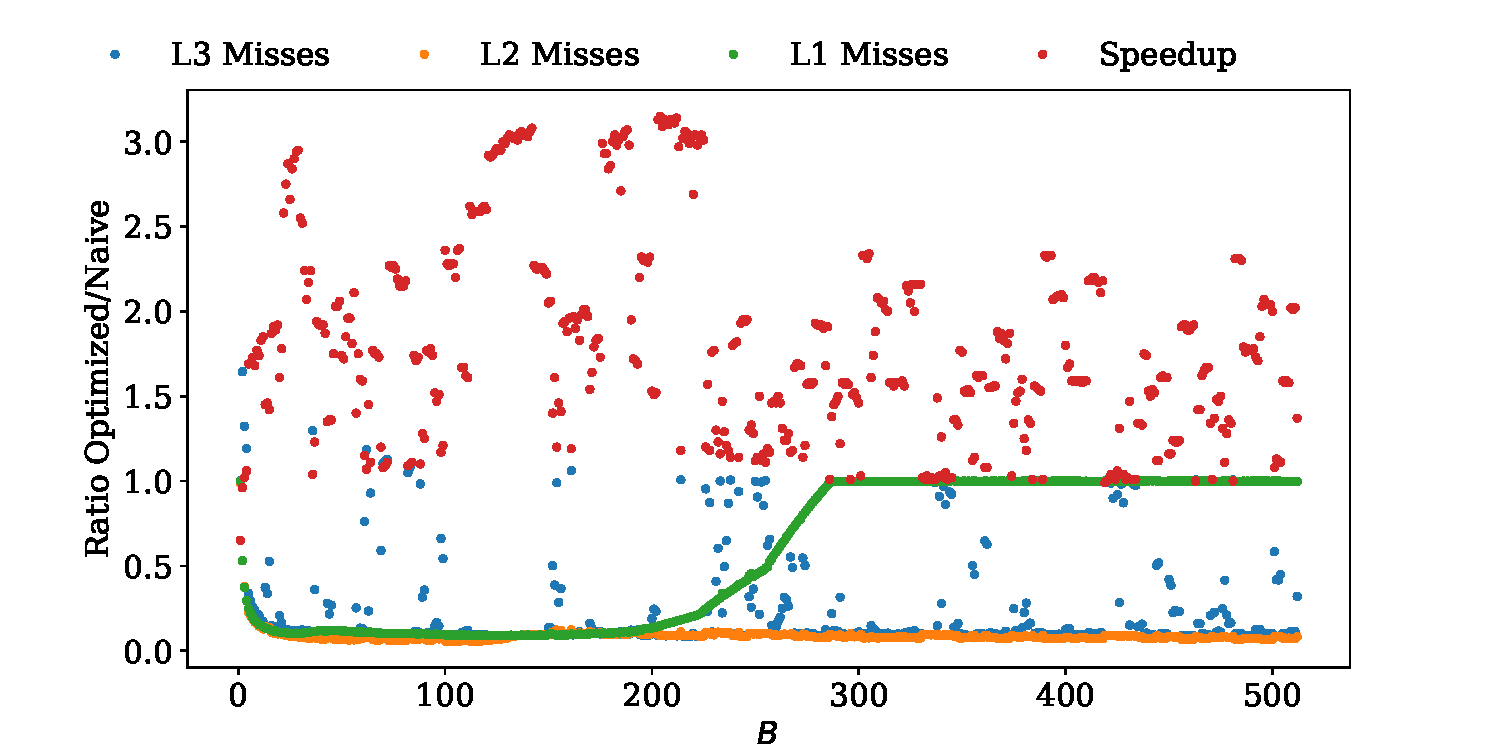
\includegraphics[width=\textwidth]{../plot/wide_against_B.pdf}
  \caption{Results for a wide matrix with $M=100000$ and $N=200$ for different blocking factors $B$.}
  \label{fig:wide_against_B}
\end{figure}

\begin{figure}
  \centering
  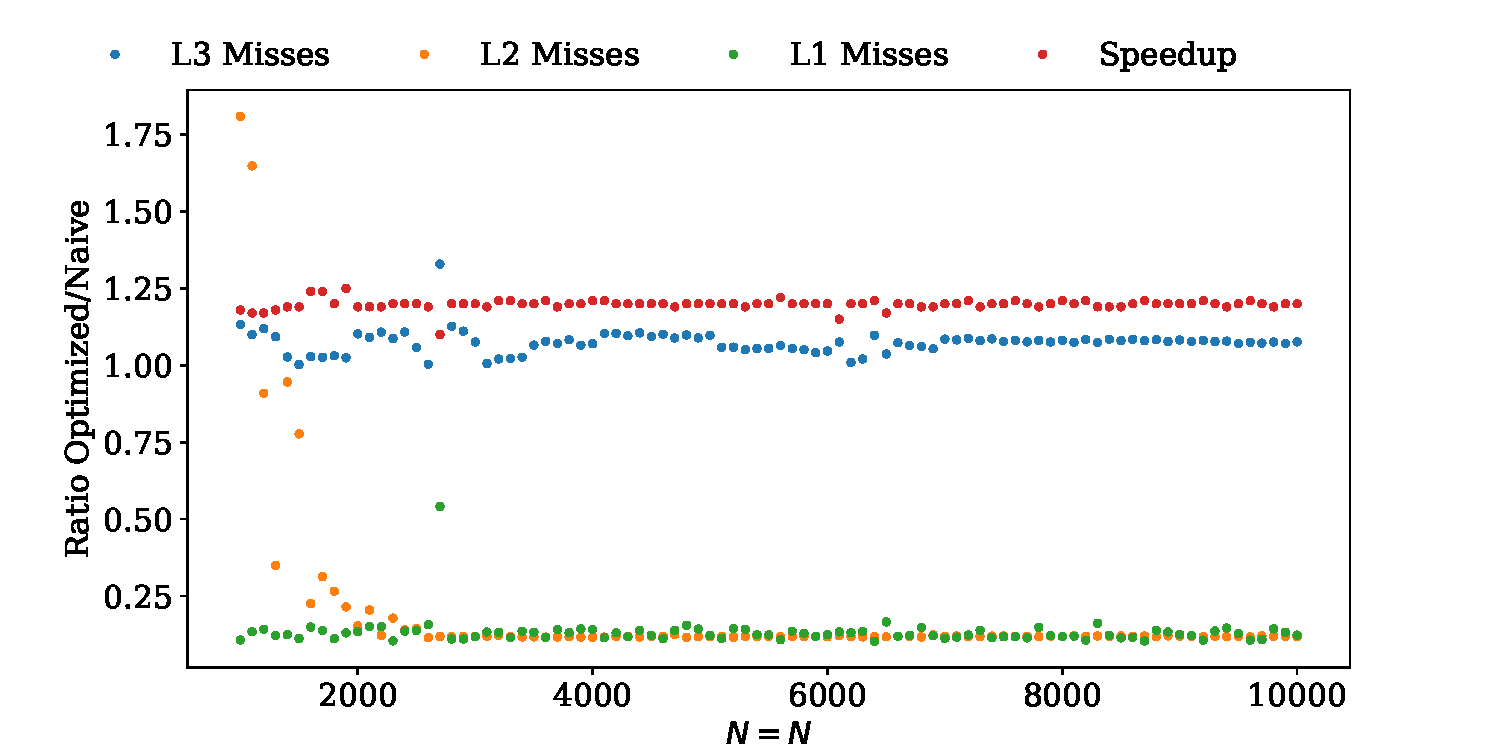
\includegraphics[width=\textwidth]{../plot/fixed_B_different_squares.pdf}
  \caption{Results for a fixed blocking factor of $B=200$ for different square matrices ($N = m$).}
  \label{fig:fixed_B_different_squares}
\end{figure}

\begin{figure}
  \centering
  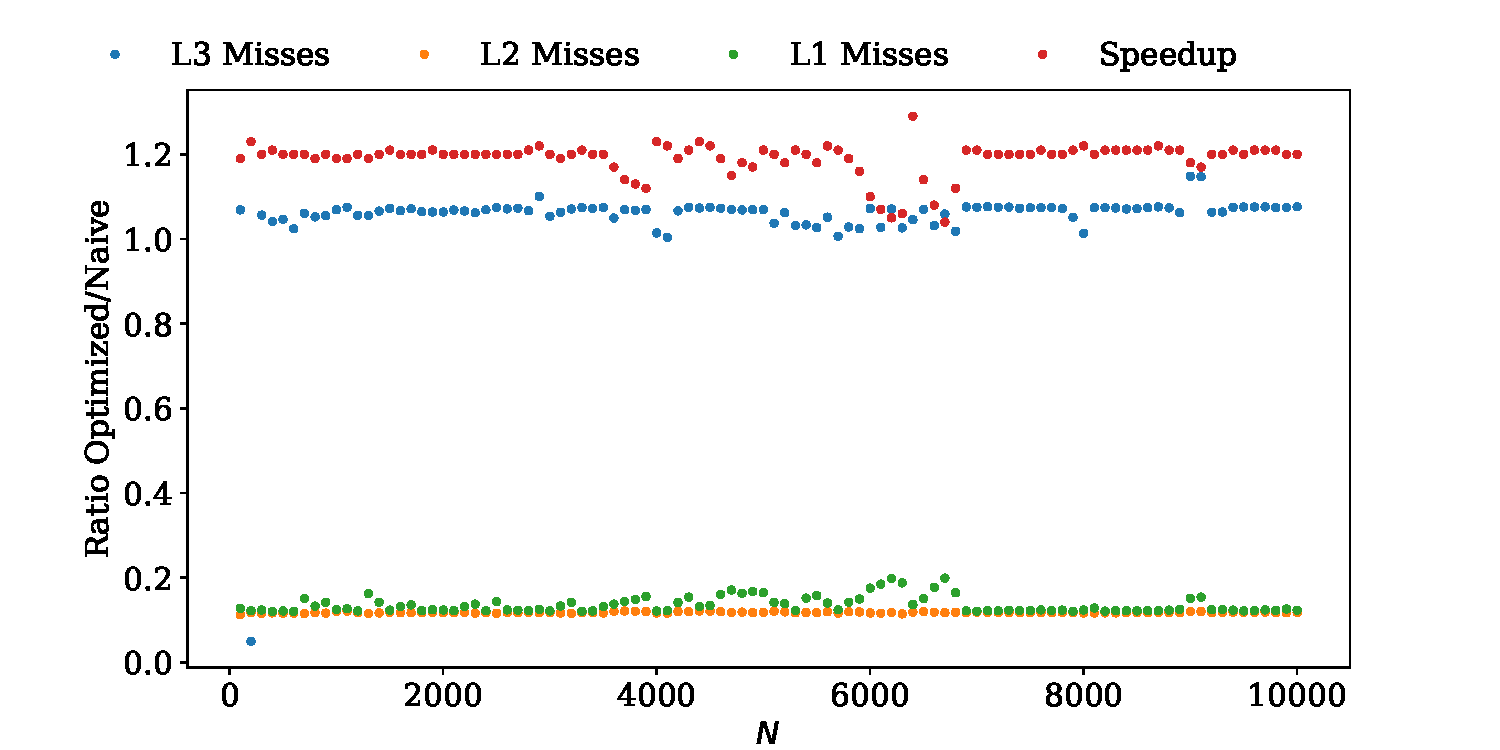
\includegraphics[width=\textwidth]{../plot/fixed_B_M_different_N.pdf}
  \caption{Results for a fixed blocking factor of $B=200$ and fixed $M=10000$
  for different $N$.}
  \label{fig:fixed_B_M_different_N}
\end{figure}

\begin{figure}
  \centering
  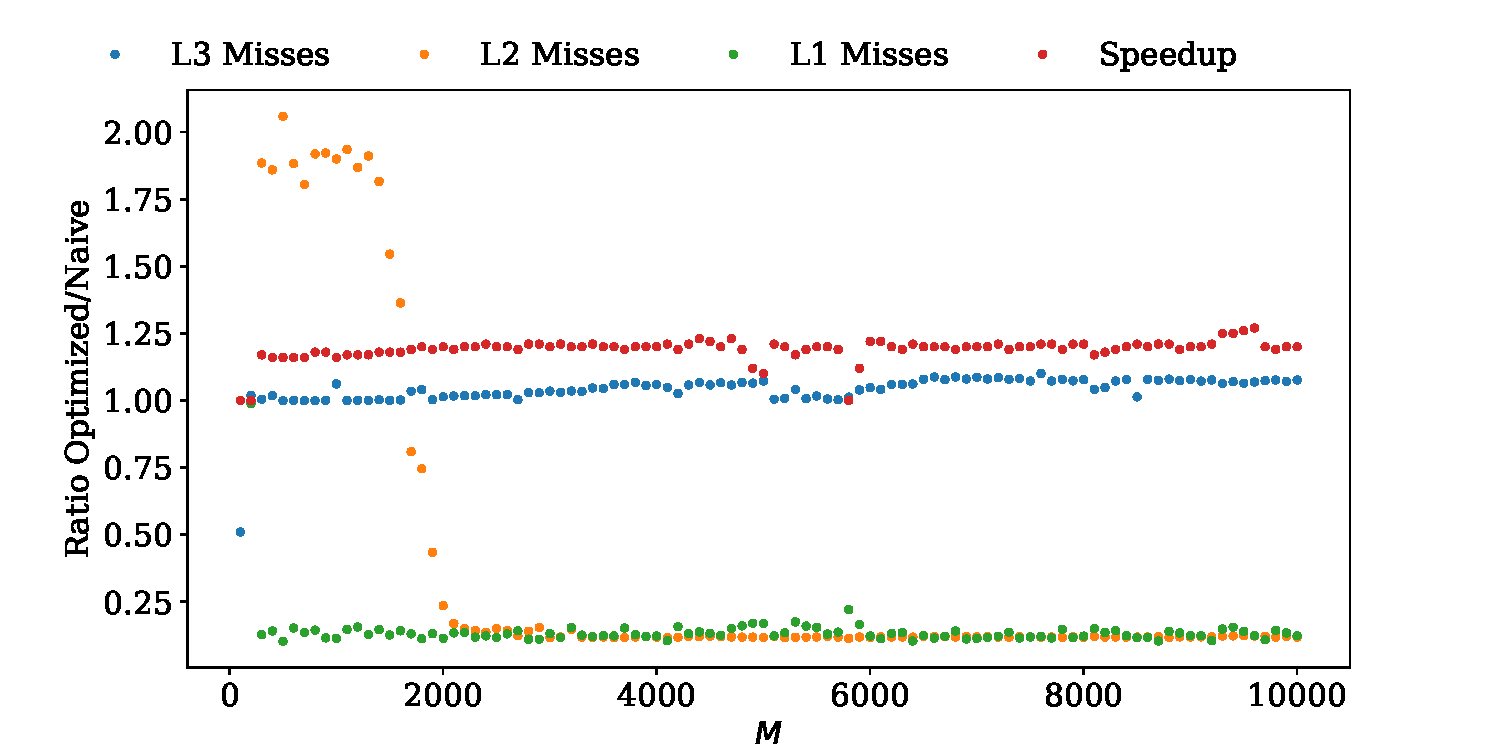
\includegraphics[width=\textwidth]{../plot/fixed_B_N_different_M.pdf}
  \caption{Results for a fixed blocking factor of $B=200$ and fixed $N=10000$
  for different $M$.}
  \label{fig:fixed_B_N_different_M}
\end{figure}

\FloatBarrier
The data visualized in Figure~\ref{fig:fixed_B_different_squares},
Figure~\ref{fig:fixed_B_M_different_N} and
Figure~\ref{fig:fixed_B_N_different_M} leads to conclude that for sufficiently
large matrices and a reasonable blocking factor, there is no correlation
between matrix shape or matrix size and performance. The performance of the
optimized implementation is consistently and significantly better than the
naive implementation.

However, we can observe significant differences for the two extreme cases
tested which are visualized in Figure~\ref{fig:narrow_against_B} and
Figure~\ref{fig:wide_against_B}. For the extreme case of a very narrow matrix
shown in Figure~\ref{fig:narrow_against_B} the optimized implementation
underperforms (probably due to added overhead by the additional loops) until
the block size approaches the width of the matrix, in which case both
implementations are equivalent (also for block sizes larger than the width). We
observe interesting behaviour in L1 and L2 miss rates for blocking factors
smaller than the matrix width: The L2 cache miss rate increases roughly by the
same factor the L1 miss rate decreases. This might be due to suboptimal branch
prediction for this scenario.

The special case of an extremely wide matrix demonstrated by
Figure~\ref{fig:wide_against_B} shows extreme performance of the optimized
implementation with speedups of over a factor of 3 for some cases. The L1 and
L2 miss rate behavior is the same observed for sufficiently large square
matrices. Additionally, here we also observe significantly lower L3 miss rates
which seem to be the cause for the large speedup factors as as the L3 miss rate
shows a negative correlation with speedup. However, I can not make out a clear
pattern, the behavior is very irregular. This is most likely due to low
statistics. The matrix is comparably small and randomly initialized. This test
should probably be repeated several times to draw conclusions from the averages
instead of single runs. The general trend is easy to explain though: The
optimized implementation works its way through the entire input matrix and
input vector block in blocks form left to right, never requiring the first
values again while the naive method works at one row of the input matrix at a
time. In the case of very few and long rows every row reaches the L3 cache
capacity which explains the observed behavior.

Therefore, in the special case of extremely rectangular matrices, it might make
sense to always transpose very narrow matrices first to always work with
extremely wide matrices instead to achieve the  performance advantage of the
optimized implementation.

The assignment also asks to make an estimation on the relative L1 and L2
latencies based on the performance and cache misses data. I do not observe a
correlation between L2 misses and performance in the data I have collected, but
I do find a strong correlation between L1 cache misses and performance.
Therefore I can not give a precise estimate on the relative latencies, I can
only say that the L1 latency is negligible when compared to the L2 latency,
which means the L2 latency is probably at least one order of magnitude larger
than the L1 latency.

\FloatBarrier
\subsection*{d) Inference about the Memory Hierarchy}
The CPUs used here are Xeon E5-2680 v4 by Intel. It has 14 cores. Each core has
448 KiB of L1 cache divided into 14 blocks of 32 KiB. The L2 cache consists of
14 256 KiB blocks adding up to a total of 3.5 MiB. The L3 cache is ten times
that large, 35 MiB consisting of 14 2.5 MiB blocks.

To make more sense of the data and use it to learn about the memory hierarchy,
we need to look at the optimized implementation and think about how many double
precision numbers are repeatedly used (and therefore potentially kept in fast
memory).

The three most inner loops with loop variables $k$, $j$ and $i$ loop over the
respective entries within a block for blocking factor $B$. The two outer loops
move the block. Considering a fixed block, so only the three most inner loops,
the algorithm repeatedly accesses 16 numbers in the output vector block, $B^2$
numbers in the input matrix and $16B$ numbers in the input vector block. That
means ideally we would like all
\begin{equation}
  N = B^2 + 16(B + 1)
  \label{eqn:L1_size}
\end{equation}
numbers to be available in
the fastest memory. Therefore, we should see a significant drop in speedup when
the critical value for B is reached, at which the L1 cache can not hold all of
these numbers anymore.

This is exactly what we observe. As discussed in the previous section,
Figure~\ref{fig:square_against_B} shows a significant drop in speedup for
$B=228$, which is where we start to see a significant increase in L1 cache
misses. That means for $B=228$ we reach the L1 cache capacity. Plugging that
into \eqref{eqn:L1_size} leads to an inferred cache capacity of $N = 55,648$
double precision floating point numbers. The double precision used here is
\SI{8}{byte}, therefore the inferred L1 cache size is roughly $55,648\cdot
\SI{8}{byte} = 445.184\,\textup{KiB}$. This is in perfect agreement with the
hardware specifications. For $B=229$ we already exceed the L1 capacity with
$N=56,121$ which would require a cache size of \SI{448.968}{KiB}.

To infer the L2 cache size we take the observed middle of the rising edge for
L2 cache misses from Figure~\ref{fig:square_against_B_L2} at $B=2083$. Plugging
that into \eqref{eqn:L1_size} results in $N = 4,372,233$ which means we can
estimate the L2 cache size to be about \SI{35}{MiB}, which again is in perfect
agreement with the given hardware specifications.

\end{document}
